\documentclass[./Differential Equations.tex]{subfiles}

\begin{document}
	\section{Definition of the Laplace Transform}
		Differentiation and integration are \textit{transforms}, meaning that, roughly speaking, these operations transform a function into another function. Moreover, these two transforms possess the \textbf{linearity property} that a transform of linear combinations of functions is a linear combination of their transforms. For two constants \(\alpha\) and \(\beta\),
			\[
				\dv{x}[\alpha f(x) + \beta g(x)] = \alpha f'(x) + \beta g'(x) \qquad \text{and} \qquad
				\int[\alpha f(x) + \beta g(x)]\dd{x} = \alpha\int f(x)\dd{x} + \beta\int g(x)\dd{x}
			\]
			provided that each derivative and integral exists. The \textbf{Laplace transform} is a special type of integral transform that has several interesting properties in addition to linearity.
		\subsectionb{Integral Transform}
			If \(f(x, y)\) is a function of two variables, a definite integral of \(f\) with respect to one of those variables results in a function of the other variable:
				\[\int_a^b f(x, y)\dd{x} = g(y)\]
				A definite integral such as
				\[\int_a^b K(s, t)f(t)\dd{t}\]
				similarly transforms a function \(f\) of variable \(t\) into a function \(F\) of variable \(s\). An \textbf{integral transform}, where the interval of integration is \([0, \infty)\), is of particular interest. If \(f(t)\) is defined for \(t \ge 0\), then
				\[\int_0^\infty K(s, t)f(t)\dd{t} = \lim_{b \to \infty}\int_0^b K(s, t)f(t) \dd{t}\]
				If this limit exists, the integral exists or is \textbf{convergent}; otherwise, it does not exist or is \textbf{divergent}. The above limit generally exists only for specific values of \(s\) (which is henceforth assumed to be a real variable).
		\subsectionb{A Definition}
			The function \(K(s, t)\) is referred to as the \textbf{kernel} of the transform. The choice \(K(s, t) = \en^{-st}\) yields an especially important integral transform.
			\callout{16.28}{\paragraph{Definition 7.1.1 Laplace Transform}
				Let \(f\) be a function defined for \(t \ge 0\). The integral
					\[\Ell\{f(t)\} = \int_0^\infty \en^{-st}f(t)\dd{t}\]
					is said to be the \textbf{Laplace transform} of \(f\), provided it converges.
			}
			When the Laplace transform converges, the resultant function \(s\) is generally denoted as the uppercase form of the lowercase letter used to denote the function of \(t\) on which the transform was performed. \\
			The domain of \(F(s)\) is dependent on \(f(t)\). \\
			The notation
			\[]_0^\infty\]
			is used as shorthand for
			\[\lim_{b\to\infty}[\,]_0^b\]
		\subsectionb{\(\mathscrbf{L}\) Is a Linear Transform}
			For a linear combination of functions,
				\[\int_0^\infty \en^{-st}[\alpha f(t) + \beta g(t)]\dd{t} = \alpha\int_0^\infty \en^{-st}f(t)\dd{t} + \beta\int_0^\infty \en^{-st}g(t)\dd{t}\]
				whenever both integrals converge for \(s > c\). It then follows that
				\[\Ell\{\alpha f(t) + \beta g(t)\} = \alpha F(s) + \beta G(s)\]
				Due to this property, \(\Ell\) is said to be a \textbf{linear transform}.
			\callout{14}{\paragraph{Theorem 7.1.1 Transforms of Some Basic Functions}
				\[\def\arraystretch{3}\begin{array}{|c|*{7}{c}|}\hline
					f(t) & 1 & t^n & \en^{\alpha t} & \sin(kt) & \cos(kt) & \sinh(kt) & \cosh(kt) \\\hline
					\Ell\{f(t)\} & \dfrac{1}{s} & \dfrac{n!}{s^{n + 1}}, n \in \Z^+ & \dfrac{1}{s - a} & \dfrac{k}{s^2 + n^2} & \dfrac{s}{s^2 + k^2} & \dfrac{k}{s^2 - k^2} & \dfrac{s}{s^2 - k^2} \\\hline
				\end{array}\]
			}
		\subsectionb{Sufficient Conditions for Existence of \(\mathscrbf{L}\)\{\textit{f}(\textit{t})\}}
			The Laplace transform's integral does not necessarily converge. Sufficient conditions to guarantee the existence of \(\Ell\{f(t)\}\) are that \(f\) be piecewise continuous on \([0, \infty)\) and that \(f\) be of exponential order for \(t > T\). A function is \textbf{piecewise continuous} on \([0, \infty)\) if for any interval \(0 \le a \le t \le b\), there are at most a finite number of points \(t_k\) at which \(f\) has finite discontinuities and is continuous on each open interval \((t_{k - 1}, t_k)\).
			\callout{17}{\paragraph{Definition 7.1.2 Exponential Order}
				A function \(f\) is said to be of \textbf{exponential order} if their eists constants \(c\), \(M > 0\) and \(T > 0\) such that \(|f(t)| \le M\en^{c^t}\) for all \(t > T\).
			}
			If \(f\) is \textit{increasing}, this simply means that on the interval \((T, \infty)\), \(f\) must not increase faster than \(M\en^{ct}\), where \(c > 0\). \\
			A positive integral power of \(t\). is always of exponential power, as for \(c > 0\),
				\[
					|t^n| \le M\en^{ct} \qquad \text{or} \qquad
					\left|\frac{t^n}{\en^{ct}}\right| \le M \quad \text{for} \quad t > T
				\]
				is equivalent to showing that
				\[\lim_{t\to\infty} \frac{t^n}{\en^{ct}}\]
				is finite for \(n \in \Z+\). The result follows from \(n\) applications of L\^opital's rule.
			\callout{17}{\paragraph{Theorem 7.1.2 Sufficient Conditions for Existence}
				If \(f\) is piecewise continuous on \([0, \infty)\) and of exponential order, then \(\Ell\{f(t)\}\) exists for \(s > c\).
			}
			By the additive property of definite integrals,
				\[
					\Ell\{f(t)\} = \int_0^T\en^{-st}f(t)\dd{t} + \int_T^\infty\en^{-st}f(t)\dd{t}
					 	= I_1 + I_2
				\]
				The integral \(I_1\) exists, as it can be written as a sum of integrals over intervals over which \(\en^{-st}f(t)\) is continuous. As \(f\) is of exponential order, there exist constants \(c\), \(M > 0\), \(T > 0\) such that \(|f(t)| \le M\en^{ct}\) for \(t > T\). It can then be written that
				\[
					|I_2| \le \int_T^\infty |\en^{-st}f(t)|\dd{t}
						\le M\int_T^\infty \en^{-st}\en^{ct}\dd{t}
						= M\int_T^\infty \en^{(-s - c)t}\dd{t} 
						= M\frac{\en^{(-s - c)T}}{s - c}
				\]
				for \(s > c\). As \(\int_T^\infty M\en^{-(s - c)t} \dd{t}\) converges, so must \(\int_T^\infty \en^{-st}f(t)\dd{t}\) by the comparison test for improper integrals. As both \(I_1\) and \(I_2\) exist, so does \(\Ell\{f(t)\}\).
			\callout{8.7}{\paragraph{Theorem 7.1.3 Behavior of \(\bm{F(s)}\) as \(\bm{s \to \infty}\)}
				If \(F(s) = \Ell\{f(t)\}\) exists, then \(\lim_{s \to \infty} F(s) = 0\).
			}
				As \(f\) is of exponential order, there exist constants \(\gamma\) and \(M_1, T \in \R^+\) such that \(|f(t)| \le M_1\en^{\gamma t}\) for \(t > T\). As \(f\) is piecewise continuous over \([0, T]\), it must be bounded on that interval; that is, \(|f(t)| \le M_2 = m_2\en^{0t}\). If \(M = \max\{M_1, M_2\}\) and  \(c = \max\{0, \gamma\}\), then
				\[
					|F(s)| \le \int_0^\infty \en^{-st}|f(t)|\dd{t}
						\le M\int_0^\infty \en^{-st}\en^{ct}
						= M\int_0^\infty \en^{-(s - c)t}\dd{t}
						= \frac{M}{s - c}
				\]
				for \(s > c\). As \(s \to \infty\), the denominator also goes to \(\infty\), so \(|F(s)| \to 0\), so \(F(s) = \Ell\{f(t)\} \to 0\).
	\section{Inverse Transforms and Transforms of Derivatives}
		\subsection{Inverse Transforms}
			\subsubsectionb{The Inverse Problem}
				If \(F(s) = \Ell\{f(t)\}\), is can be said that \(f(t)\) is the \textbf{inverse Laplace transform} of \(F(s)\), denoted
					\[f(t) = \Ell^{-1}\{F(s)\}\]
				\callout{14}{\paragraph{Theorem 7.2.1 Some Inverse Transforms}
					\[\def\arraystretch{3}\begin{array}{|c|*{7}{c}|}\hline
						F(s) & \dfrac{1}{s} & \dfrac{n!}{s^{n + 1}}, n \in \N & \dfrac{1}{s - a} & \dfrac{k}{s^2 + k^2} & \dfrac{s}{s^2 + k^2} & \dfrac{k}{s^2 - k^2} & \dfrac{s}{s^2 - k^2} \\\hline
						\Ell^{-1}\{F(s)\} & 1 & t^n & \en^{at} & \sin(kt) & \cos(kt) & \sinh(kt) & \cosh(kt) \\\hline
					\end{array}\]
				}
			\subsubsectionb{\(\mathscrbf{L}\) is a Linear Transform}
				The inverse Laplace transform is also linear; that is,
					\[\Ell^{-1}\{\alpha F(s) + \beta G(s)\} = \alpha\Ell^{-1}\{F(s)\} + \beta\Ell^{-1}\{G(s)\}\]
					for some constants \(\alpha\) and \(\beta\).
			\subsubsectionb{Partial Fractions}
				Decomposing a function into its partial fractions is often useful in evaluating its inverse Laplace transform. 
		\subsection{Transforms of Derivatives}
			\subsubsectionb{Transform a Derivative}
				If \(f'\) is continuous, integration by parts gives
					\[
						\Ell\{f'(t)\} = \int_0^\infty \en^{-st}f'(t)\dd{t}
							= \left[\en^{-st}f(t)\right]_0^\infty + s\int_0^\infty \en^{-st}f(t)
							= -f(0) + s\Ell\{f(t)\}
					\]
					or
					\[\Ell\{f'(t)\} = sF(s) - f(0)\]
					Using this result
					\begin{align*}
						\Ell\{f''(t)\} &= \int_0^\infty \en^{-st}f''(t)\dd{t}
								= \left[\en^{-st}f'(t)\right]_0^\infty + s\int_0^\infty \en^{-st}f'(t)\dd{t} \\
							&= -f'(0) + s\Ell\{f'(t)\}
								= s[sF(s) - f(0)] - f'(0)
					\end{align*}
					or
					\[\Ell\{f''(t)\} = s^2F(s) - sf(0) - f'(0)\]
					It can similarly be shown that
					\[\Ell\{f''(t)\} = s^3F(s) - s^2f(0) - sf'(0) - f''(0)\]
				\callout{17}{\paragraph{Theorem 7.2.2 Transform of a Derivative}
					If \(f, f', \ldots, f^{(n - 1)}\) are continuous on \([0, \infty\) and of exponential order and if \(f^{(n)}(t)\) is piecewise continuous on \([0, \infty)\), then
						\[
							\Ell\left\{f^{(n)}\right\} = s^nF(s) - s^{n - 1}f(0) - s^{n - 2}f'(0) - \cdots - f^{(n - 1)}(0)
								= s^nF(s) - \sum_{i = 1}^n s^{n - i}f^{(i - 1)}(0)
						\]
						where \(F(s) = \Ell\{f(t)\}\).
				}
			\subsubsectionb{Solving Linear ODEs}
				\(\Ell\{\dv*[n]{y}{t}\}\) is evidently dependent on \(Y(s) = \Ell\{y(t)\}\) and on the \(n - 1\) derivatives of \(y(t)\) at \(t = 0\). This property makes the Laplace transform well-suited to solving linear IVPs in which the DE has \textit{constant coefficients}. Such a DE is simply a linear combination of \(y\) and its \(n\) derivatives:
					\[
						a_0\dv[n]{y}{t} + a_{n - 1}\dv[n - 1]{y}{t} + \cdots + a_0y = g(t), \qquad
							y(0) = y_0, y'(0) = y_1, \ldots, y^{(n - 1)}(0) = y_{n - 1}
					\]
					where \(a_{0 \cdots n}\) and \(y_{0 \cdots n - 1}\) are constants. By linearity, the Laplace transform of this linear combination is itself a linear combination of Laplace transforms:
					\[a_n\Ell\left\{\dv[n]{y}{t}\right\} + a_{n - 1}\Ell\left\{\dv[n - 1]{y}{t}\right\} + \cdots + a_0\Ell\{y\} = \Ell\{g(t)\}\]
					This becomes
					\[a_n\left[s^nY(s) \sum_{i = 1}^n s^{n - i}y^{(i - 1)}(0)\right] + a_{n - 1}\left[s^{n - 1}Y(s) - \sum_{i = 2}^{n}s^{(n - i)}y^{(i - 2)}\right] + \cdots + a_0Y(s) = G(s)\]
					where \(Y(s) = \Ell\{y(t)\}\) and \(G(s) = \Ell\{g(t)\}\).
					\callout{9.03}{
						\textit{The Laplace transform of a linear DE with constant coefficients becomes an algebraic equation in \(Y(s)\).}
					}
					It can be written that
					\[P(s)Y(s) = Q(s) + G(s)\]
					where
					\[P(s) = a_ns^n + a_{n - 1}s^{n - 1} + \cdots + a_0\]
					and \(Q(s)\) is a polynomial in \(s\) of degree \(\le n - 1\) comprised of the various products of the coefficients \(a_i\) and the prescribed initial conditions \(y_i\). Rewriting,
					\[Y(s) = \frac{Q(s)}{P(s)} + \frac{G(s)}{P(s)}\]
					These two terms are typically combined over the least common denominator before being composed into partial fractions. The solution \(y(t)\) is then simply \(\Ell^{-1}\{Y(s)\}\).
					\callout{17}{\paragraph{Figure 7.2.1 Steps in solving an IVP by the Laplace transform}
						\[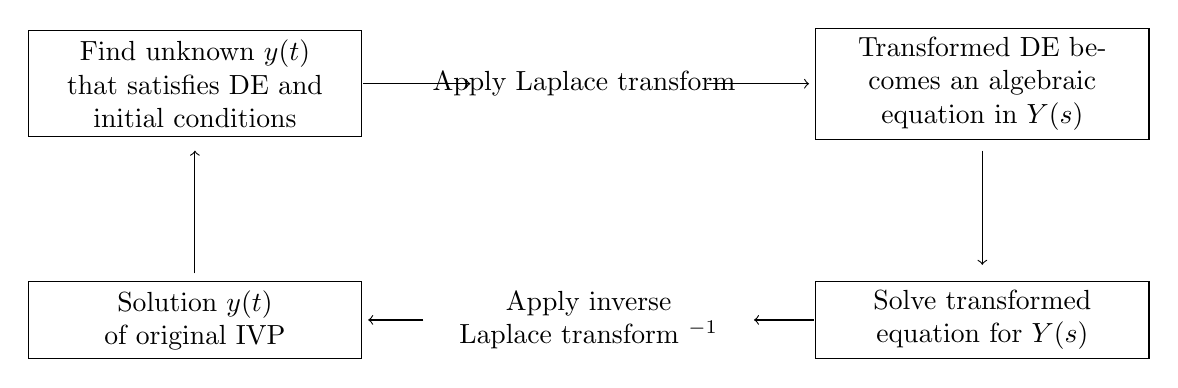
\begin{tikzpicture}
							\node at (-5, 1) [draw, align = center, text width = 4cm] {Find unknown \(y(t)\) that satisfies DE and initial conditions};
								\draw[->] (-2.86, 1) -- (-1.5, 1);
							\node at (0, 1) [align = center, text width = 4cm] {Apply Laplace transform \(\Ell\)};
								\draw[->] (1.5, 1) -- (2.8, 1);
							\node at (5, 1) [draw, align = center, text width = 4cm] {Transformed DE becomes an algebraic equation in \(Y(s)\)};
								\draw[->] (5, 0.15) -- (5, -1.3);
							\node at (5, -2) [draw, align = center, text width = 4cm] {Solve transformed equation for \(Y(s)\)};
								\draw[->] (2.86, -2) -- (2.1, -2);
							\node at (0, -2) [align = center, text width = 4cm] {Apply inverse Laplace transform \(\Ell^{-1}\)};
								\draw[->] (-2.1, -2) -- (-2.8, -2);
							\node at (-5, -2) [draw, align = center, text width = 4cm] {Solution \(y(t)\) of original IVP};
								\draw[->] (-5, -1.41) -- (-5, 0.15);
						\end{tikzpicture}\]
					}
	\section{Operational Properties I}
		\subsection{Translation on the \textit{s}-Axis}
			\subsubsectionb{A Translation}
				In general, if \(\Ell\{f(t)\} = F(s)\) is known, then \(\Ell\{\en^{at}f(t)\}\) can be computed.
				\callout{17}{\paragraph{Theorem 7.3.1 First Translation Theorem}
					If \(\Ell\{f(t)\} = F(s)\) and \(a\) is a real number, then
						\[\Ell\{\en^{at}f(t)\} = F(s - a)\]
				}
				By the definition of the Laplace transform,
				\[
					\Ell\{\en^{at}f(t)\} = \int_0^\infty \en^{-st}\en^{at}f(t)\dd{t}
						= \int_0^\infty \en^{-(s - a)t}f(t)\dd{t}
						= F(s - a)
				\]
				If \(s\) is regarded as a real variable, the graph of \(F(s - a)\) is simply the graph of \(F(s)\) shifted along the \(s\)-axis by \(|a|\). If \(a > 0\), the shift is to the right, while it is to the left if \(a < 0\). \\
				For emphasis, it is sometimes useful to use the notation
					\[\Ell\{\en^{at}f(t)\} = \Ell\{f(t)\}|_{s \to s - a}\]
					where \(s \to s - a\) means that the Laplace transform \(F(s)\) replaces \(s\) with \(s - a\) wherever it appears.
			\subsubsectionb{Inverse Form of a Translation}
				To compute the inverse of \(F(s - a)\), \(F(s)\) must be recognized. \(\Ell^{-1}\{F(s - a)\}\) is then simply the product of \(f(t) = \Ell^{-1}F(s)\) and \(\en^{at}\). Symbolically, this can be summarized as
					\[
						\Ell^{-1}\{F(s - a)\} = \Ell^{-1}\{F(s)|_{s \to s - a}\}
							= \en^{at}f(t)
					\]
		\subsection{Translation on the \textit{t}-Axis}
			\subsubsectionb{Unit Step Function}
				\callout{17}{\paragraph{Definition 7.3.1 Unit Step Function}
					The \textbf{unit step function} (or \textbf{Heaveside function}) \(\Uscr(t - a)\) is defined to be
						\[
							\Uscr(t - a) =
								\begin{cases}
									0 & 0 \le t < a \\
									1 & t \ge a	
								\end{cases}
						\]
				}
				Note that \(\Uscr(t - a)\) is defined only on the nonnegative \(t\)-axis, as this is all that must be considered when working with the Laplace transform. In a broader sense, \(\Uscr(t - a) = 0\) for all \(t < a\). \\
				When a function \(f\) defined for \(t \ge 0\) is multiplied by \(\Uscr(t - a)\), the unit step function \enquote{turns off} the portion of the graph that is before \(t = a\). \\
				The unit step function can be used to compactly write piecewise functions:
					\[
						f(t) =
							\begin{cases}
								g(t) & 0 \le t < a \\
								h(t) & t \ge a	
							\end{cases}
							= g(t) - g(t)\Uscr(t - a) + h(t)\Uscr(t - a)
					\]
					\[
						f(t) = 
							\begin{cases}
							0 & 0 \le t < a \\
							g(t) & 	a \le t < b \\
							0 & t \ge b
							\end{cases}
							= g(t)[\Uscr(t - a) - \Uscr(t - b)]
					\]
				\callout{17}{\paragraph{Theorem 7.3.2 Second Translation Theorem}	
					If \(F(s) = \Ell\{f(t)\}\) and \(a > 0\), then
						\[\Ell\{f(t - a)\Uscr(t - a)\} = \en^{-as}F(s)\]
				}
				By the additive property of integrals,
					\begin{align*}
						\Ell\{f(t - a)\Uscr(t - a)\} &= \int_0^\infty \en^{-st}f(t - a)\Uscr(t - a)\dd{t} \\
							&= \int_0^a \en^{-st}f(t - a)\underset{0 \text{ for } 0 \le t < a}{\underbrace{\Uscr(t - a)}}\dd{t} + \int_a^\infty \en^{-st}f(t - a)\underset{1 for t \ge a}{\underbrace{\Uscr(t - a)}}\dd{t} \\
							&= \int_a^\infty \en^{-st}f(t - a) \dd{t}
					\end{align*}
					Letting \(v = t - a\) and \(\dd{v} = \dd{t}\),
					\begin{align*}
						 \Ell\{f(t - a)\Uscr(t - a)\} &= \int_a^\infty \en^{-st}f(t - a) \dd{t}
						 		= \int_0^\infty \en^{-s(v + a)}f(v)\dd{v} \\
						 	&= \en^{-as}\int_0^\infty \en^{-sv}f(v)\dd{v}
						 		= \en^{-as}\Ell\{f(t)\}
					\end{align*}
				The Laplace transform of just a unit step function is
					\[\Ell\{\Uscr(t - a)\} = \frac{\en^{-as}}{s}\]
			\subsubsectionb{Inverse Transform to a Step Function}
				When \(a > 0\),
					\[\Ell^{-1}\{\en^{-as}F(s)\} = f(t - a)\Uscr(t - a)\]
			\subsubsectionb{Alternative Form}
				
\end{document}
